\section{Prediction Model}\label{prediction_model}
To learn from labelled patient dataset and be able to properly predict 
the occurence or not of Malaria given a new patient, we harness the logistic 
regression function as our \emph{classifier}. 
In this section, we briefy recall the basic of the logistic regression function
and how it can act as a binary classifier. We start by introducing the binary 
classification problem we have to solve in the study.

% binary classification problem for Malaria
\subsection{Binary classification problem}
Let us assume two given classes of Malaria diagnostic: \emph{Malaria} and \emph{Not-Malaria}.
We also consider \textsc{P} and \textsc{C} as respectively the set of patients and a prediction model.
A patient \emph{p} in \textsc{P} is defined by a set of pairs $(a_1, v_1), (a_2, v_2), \ldots, (a_n, v_n)$
where $a_i$ and $v_i$, for each $1\leq i\leq n$, respectively corresponds to a given Malaria feature and its associated value defined
as follows.
\begin{equation}
v_i = \left\{
\begin{array}{rl}
1 &\text{if $a_i$ is observed} \\
0 &\text{otherwise} \\
\end{array}
\right.
\end{equation}

\begin{definition}{(Our prediction problem)}
We define our binary classification problem for the prediction of the occurrence
or not of Malaria on a given patient dataset as a mapping \textsc{C} of every patient p in \textsc{P} 
to one and only one class in \{Malaria, Not-Malaria\}. Formally, we present such a mapping as \textsc{C}: \textsc{P} $\mapsto$ \{Malaria, Not-Malaria\}.
\end{definition}


We define and use  \textsc{C} with the help of the logistic regression for the specific purpose of our study. 
% Logistic regession function
\subsection{Logistic regression}
The logistic regression (a.k.a the logit function) is a statistical model used in the machine learning domain for binary classification.
In its basic form, it is based on a logistic function to model a binary dependent variable \cite{Sa14}.
As an input, the logistic regression  takes qualitative or/and ordinal predictive variables (e.g. the presence
or not of fever given a patient) in order to measure the probability of the outcome (e.g. the occurrence or not of the Malaria) 
by using the \emph{Sigmoid function}. Figure \ref{sigmoid_curve} shows the shape of the curve of the Sigmoid function. 

% The curve of the logistic regression
\begin{figure}[ht]
\centering
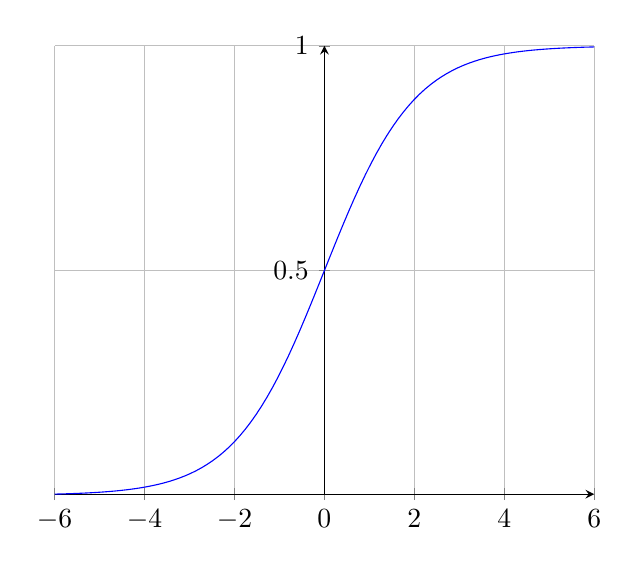
\begin{tikzpicture}
    \begin{axis}%
    [
        grid=major,     
        xmin=-6,
        xmax=6,
        axis x line=bottom,
        ytick={0,.5,1},
        ymax=1,
        axis y line=middle,
    ]
        \addplot%
        [
            blue,%
            mark=none,
            samples=100,
            domain=-6:6,
        ]
        (x,{1/(1+exp(-x))});
    \end{axis}
\end{tikzpicture}
\caption{The curve of the Sigmoid function}\label{sigmoid_curve}
\end{figure}
